\documentclass{article}
\usepackage{tkz-euclide}
\usepackage{amsmath}
\usepackage[colorlinks]{hyperref}
\title{Geometry and forces exerted on a bubble and a drop attached to each other}
\author{}
\date{\today}

\begin{document}
\maketitle

\begin{figure}
    \begin{center}
        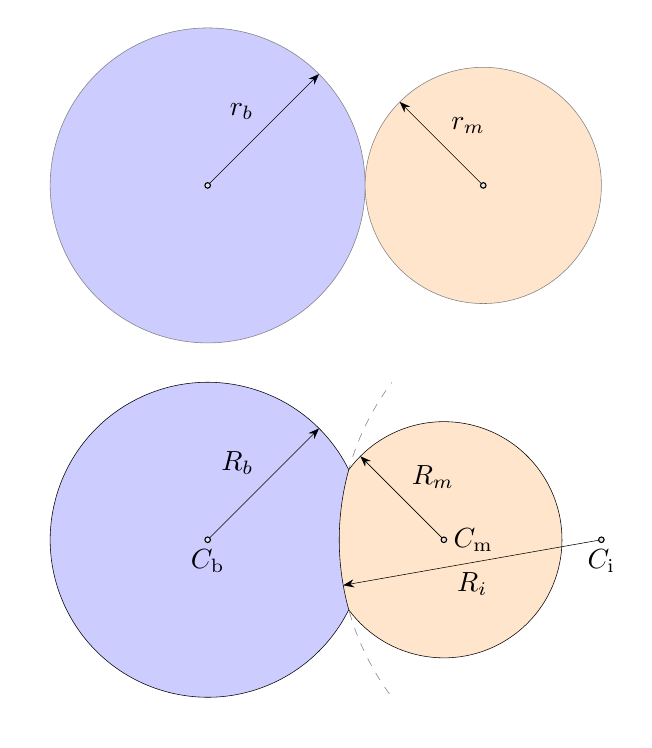
\begin{tikzpicture}
            \tkzDefPoints{0/4.5/C_b_j, 3.5/4.5/C_m_j}
            \tkzDefCircle[R](C_b_j,2)
            \tkzGetPoint{c_b_j_x}
            \tkzDrawCircle[fill=blue!20](C_b_j,c_b_j_x)
            \tkzDefPointOnCircle[through= center C_b_j angle 45 point c_b_j_x]
            \tkzGetPoint{aa}
            \tkzDrawSegment[-Stealth](C_b_j, aa)
            \tkzLabelSegment[above left](C_b_j, aa){$r_b$}
            %\tkzLabelPoint(C_b_j){$C_\text{b}$}

            \tkzDefCircle[R](C_m_j,1.5)
            \tkzGetPoint{c_m_j_x}
            \tkzDrawCircle[fill=orange!20](C_m_j,c_m_j_x)
            \tkzDefPointOnCircle[through= center C_m_j angle 135 point c_m_j_x]
            \tkzGetPoint{bb}
            \tkzDrawSegment[-Stealth](C_m_j, bb)
            \tkzLabelSegment[above right](C_m_j, bb){$r_m$}
            %\tkzLabelPoint[right](C_m_j){$C_\text{m}$}

            %%%%%%%%%%%%%%%%%%%%
            \tkzDefPoint(0,0){C_b}
            \tkzDefCircle[R](C_b,2)
            \tkzGetPoint{c_b_x}

            \tkzDefPoint(3,0){C_m}
            \tkzDefCircle[R](C_m,1.5)
            \tkzGetPoint{c_m_x}

            \tkzInterCC(C_b,c_b_x)(C_m,c_m_x)
            \tkzGetPoints{I}{J}
            %\tkzLabelPoints(I,J)
            %\tkzDrawPoints(I,J)

            \tkzDefPoint(5,0){C}
            \begin{scope}
                \tkzDefPoints{0/-2/AA,5/-2/BB,5/2/CC,0/2/DD}
                \tkzClipPolygon(AA,BB,CC,DD)
                \tkzDrawCircle[dashed](C,I)
            \end{scope}

            \tkzDrawArc[fill=blue!20](C_b,I)(J)
            \tkzDrawArc[fill=orange!20](C_m,J)(I)
            \tkzDrawArc[fill=orange!20](C,I)(J)

            %\tkzDrawSegment[-Stealth](C_b,I)
            %\tkzLabelSegment[above](C_b,I){$R^0_\text{b}$}
            %\tkzDrawSegment[-Stealth](C_m,I)
            %\tkzLabelSegment[below](C_m,I){$R^0_\text{m}$}
            %\tkzDrawSegment[-Stealth](C,I)
            %\tkzLabelSegment[above](C,I){$R_\text{i}$}
            %\tkzDrawSegment(C_b,C)


            \tkzDefPointOnCircle[through= center C_b angle 45 point c_b_x]
            \tkzGetPoint{cc}
            \tkzDrawSegment[-Stealth](C_b, cc)
            \tkzLabelSegment[above left](C_b, cc){$R_b$}

            \tkzDefPointOnCircle[through= center C_m angle 135 point c_m_x]
            \tkzGetPoint{dd}
            \tkzDrawSegment[-Stealth](C_m, dd)
            \tkzLabelSegment[above right](C_m, dd){$R_m$}

            \tkzDefPointOnCircle[through= center C angle 190 point I]
            \tkzGetPoint{ee}
            \tkzDrawSegment[-Stealth](C, ee)
            \tkzLabelSegment[below](C, ee){$R_i$}

            \tkzDrawPoints(C_b, C_m, C, C_b_j, C_m_j)
            \tkzLabelPoint(C_b){$C_\text{b}$}
            \tkzLabelPoint[right](C_m){$C_\text{m}$}
            \tkzLabelPoint(C){$C_\text{i}$}
        \end{tikzpicture}
    \end{center}
    \caption{
        A bubble of gas (blue)  and a drop of molten metal (orange) in a 
        liquid, right before attachment (top) and after (bottom).
    }\label{fig:one}
\end{figure}

We consider a bubble of fluid (labelled by the letter b) and a drop of molten
metal (label m) floating in a liquid (label l). Before attachment, 
the bubble has a radius of $R^0_\text{b}$ and the drop of $R^0_\text{m}$, (fig.~\ref{fig:one}, top).
By attaching to each other (and once equilibrium is reached), an interface forms between them (label i), 
that can intrude into the bubble (as depicted in fig.~\ref{fig:one}, bottom) or into the drop.
%The bubble, drop and interface are considered spherical. 
The bubble now has a radius
$R^0_\text{b}$, the drop $R^0_\text{m}$ and the interface between them, $R_\text{i}$. 
The pressures inside the bubble, drop and bulk liquid are
$P_\text{b}$, $P_\text{m}$ and $P_\text{l}$, respectively. The surface tensions
between the fluids are $\sigma_\text{bm}$, $\sigma_\text{bl}$, and
$\sigma_\text{ml}$. 

By the Young-Laplace equation
\begin{align}
    P_\text{b} - P_\text{l} &= 2\frac{\sigma_\text{bl}}{R^0_\text{b}}
    \label{eq:yl-b}
    ,\\
    P_\text{m} - P_\text{l} &= 2\frac{\sigma_\text{ml}}{R^0_\text{m}}
    \label{eq:yl-m}
    ,\\
    \left| P_\text{m} - P_\text{b} \right| &= 2\frac{\sigma_\text{bm}}{R_\text{i}}
    \label{eq:yl-i}
    .
\end{align}
(This assumes that $P_\text{b}>P_\text{l}$ and $P_\text{m}>P_\text{l}$,
but nothing about the magnitude of $P_\text{m}$ relatively to $P_\text{b}$.)
By substituting eq.~\ref{eq:yl-b} and eq.~\ref{eq:yl-m} into eq.~\ref{eq:yl-i}
\begin{equation}
    R_\text{i} = \frac
        {R^0_\text{m}R^0_\text{b}\sigma_\text{bm}}
        {\left| R^0_\text{b}\sigma_\text{bl} - R^0_\text{m}\sigma_\text{ml} \right| }
        \label{eq:ri}
\end{equation}
(Note that if $R^0_\text{b}=R^0_\text{m}$ and $\sigma_\text{bl} = \sigma_\text{ml}$,
then $R\rightarrow \infty$. In other words if the bubble and drop have the same
size and the surface tensions are equal, then the interface is flat.)
The sign of the difference $(R^0_\text{b}\sigma_\text{bl} - R^0_\text{m}\sigma_\text{ml})$ tells us 
whether the interface intrudes into the bubble (if positive) or into the drop 
(if negative). If its value is zero, the interface is flat.


\begin{figure}
    \begin{center}
        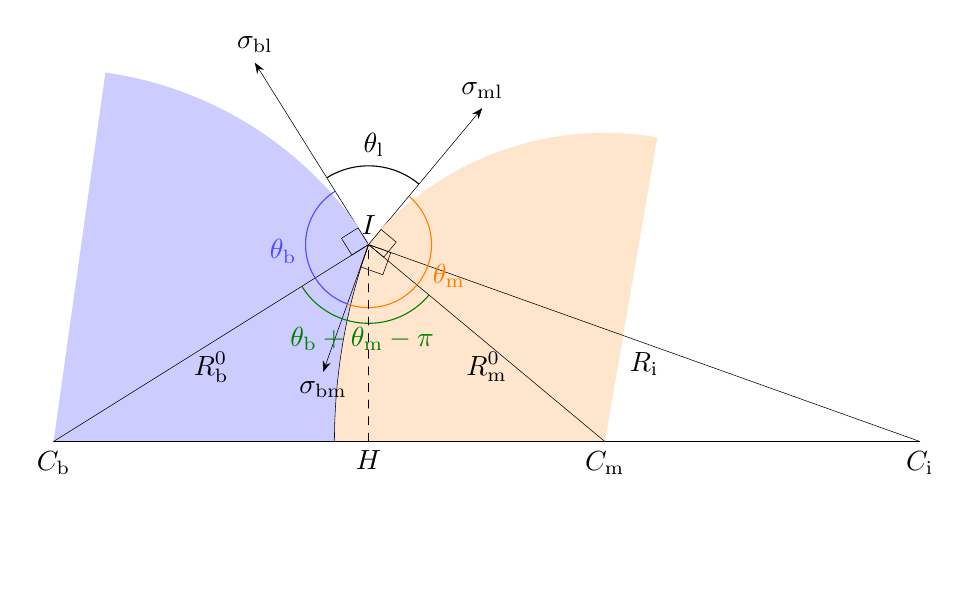
\begin{tikzpicture}
            \tkzDefPoint(0,0){C_b}
            \tkzLabelPoint(C_b){$C_\text{b}$}
            \tkzDefPoint(7,0){C_m}
            \tkzLabelPoint(C_m){$C_\text{m}$}
            \tkzDefPoint(11,0){C_i}
            \tkzLabelPoint(C_i){$C_\text{i}$}
            \tkzDefPoint(4,2.5){I}
            \tkzLabelPoint[above](I){$I$}

            \tkzDefTriangle[school](C_b,I)
            \tkzGetPoint{st_b}
            \tkzLabelPoint[above](st_b){$\sigma_\text{bl}$}
            \tkzDefPointBy[rotation= center C_b angle 50](I)
            \tkzGetPoint{arc_b}
            \tkzDefTriangle[school,swap](C_m,I)
            \tkzGetPoint{st_m}
            \tkzLabelPoint[above](st_m){$\sigma_\text{ml}$}
            \tkzDefPointBy[rotation= center C_m angle -60](I)
            \tkzGetPoint{arc_m}

            \tkzInterLC(C_b,C_i)(C_m,I)
            \tkzGetFirstPoint{yop2}
            \tkzFillSector[fill=orange!20](C_m,arc_m)(yop2)
            \tkzInterLC(C_b,C_i)(C_b,I)
            \tkzGetSecondPoint{yop1}
            \tkzFillSector[fill=blue!20](C_b,yop1)(arc_b)

            \begin{scope}
                \tkzClipPolygon(C_b,C_m,arc_m,arc_b)
                \tkzInterLC(C_b,C_i)(C_i,I)
                \tkzGetFirstPoint{yop3}
                \tkzFillSector[fill=orange!20](C_i,I)(yop3)
            \end{scope}

            \tkzDrawSegments(C_b,C_i C_b,I C_m,I C_i,I)

            \tkzDrawSegment[-Stealth](I,st_b)
            \tkzDrawArc[blue!20,thick](C_b,I)(arc_b)
            \tkzMarkRightAngle[very thin](C_b,I,st_b)

            \tkzDrawSegment[-Stealth](I,st_m)
            \tkzDrawArc[orange!20,thick](C_m,arc_m)(I)
            \tkzMarkRightAngle[very thin](C_m,I,st_m)

            \tkzDefTriangle[school](C_i,I)
            \tkzGetPoint{x}
            \tkzDefPointOnLine[pos=0.4](I,x)
            \tkzGetPoint{st_i}
            \tkzLabelPoint[below](st_i){$\sigma_\text{bm}$}
            \tkzDrawSegment[-Stealth](I,st_i)
            \tkzInterLC(C_b,C_i)(C_m,I)
            \tkzGetFirstPoint{arc_m}
            \tkzDrawArc(C_i,I)(arc_m)
            \tkzMarkRightAngle[very thin,size=.3](C_i,I,st_i)

            \tkzMarkAngle[size=1](st_m,I,st_b)
            \tkzLabelAngle[above](st_m,I,st_b){$\theta_\text{l}$}
            \tkzMarkAngle[size=0.8,blue!70](st_b,I,st_i)
            \tkzLabelAngle[pos=0.8,left](st_b,I,st_i){\color{blue!70}$\theta_\text{b}$}
            \tkzMarkAngle[size=0.8,orange](st_i,I,st_m)
            \tkzLabelAngle[pos=0.8,right](st_i,I,st_m){\color{orange}$\theta_\text{m}$}
            %\tkzMarkAngle[size=1.4](C_b,I,C_i)
            %\tkzLabelAngle[pos=1.7](C_b,I,C_i){$\theta_\text{b}$}
            \tkzMarkAngle[size=1,green!50!black](C_b,I,C_m)
            \tkzLabelAngle[pos=1.2](C_b,I,C_m){\color{green!50!black}$\theta_\text{b}+\theta_\text{m}-\pi$}

            \tkzLabelSegment(C_b,I){$R^0_\text{b}$}
            \tkzLabelSegment(C_m,I){$R^0_\text{m}$}
            \tkzLabelSegment(C_i,I){$R_\text{i}$}

            \tkzDefPointBy[projection= onto C_b--C_i](I)
            \tkzGetPoint{H}
            \tkzLabelPoint(H){$H$}
            \tkzDrawSegment[dashed](H,I)

        \end{tikzpicture}
    \end{center}
    \caption{Zoom on the contact between the bubble and the drop}\label{fig:two}
\end{figure}

The contact angles in the bubble, drop and surrounding liquid are
$\theta_\text{b}$, $\theta_\text{m}$ and $\theta_\text{l}$, respectively
(fig.~\ref{fig:two}).
At equilibrium, the surface tensions and the contact angles are related by
\begin{align}
    \cos{\sigma_\text{b}} &= \frac
    {\sigma_\text{ml}^2 - \sigma_\text{bl}^2 - \sigma_\text{bm}^2}
    {2\sigma_\text{bl}\sigma_\text{bm}}
    ,\\
    \cos{\sigma_\text{m}} &= \frac
    {\sigma_\text{bl}^2 - \sigma_\text{bm}^2 - \sigma_\text{ml}^2}
    {2\sigma_\text{bm}\sigma_\text{ml}}
    ,\\
    \cos{\sigma_\text{l}} &= \frac
    {\sigma_\text{bm}^2-\sigma_\text{ml}^2 - \sigma_\text{bl}^2}
    {2\sigma_\text{bl}\sigma_\text{mm}}
    .
\end{align}


The $\angle C_\text{b} I C_\text{m}$ angle is equal to $\alpha - \pi$ with
\begin{equation}
    \alpha = \theta_\text{b}+\theta_\text{m}
    \label{eq:alpha}
\end{equation}
Thus, of the triangle
$(C_\text{b},I,C_i)$ we know two sides ($R^0_\text{b}$ and $R_i$) and one angle. By the law of 
cosine, the length of the segment $C_\text{b}C_\text{m}$, noted $c$, is
\begin{equation}
    c \equiv C_\text{b}C_\text{m} =  \sqrt{\left(R^0_\text{b}\right)^2 +
        \left(R^0_\text{m}\right)^2 + 2R_\text{b}R^0_\text{m}\cos{\alpha})},
    \label{eq:c2}
\end{equation}
and the area of the triangle is 
\begin{equation}
    S = -\frac{1}{2}R^0_\text{b}R^0_\text{m}\sin{\alpha}.
    \label{eq:S2}
\end{equation}
The altitude of the triangle from the vertex $I$ is noted $a$
\begin{equation}
    a \equiv IH = 2\frac{S}{c}.
    \label{eq:a-}
\end{equation}
We will need the square of that, that is
\begin{equation}
    a^2 =
    -\frac{1}{2}
    \frac
    {\left(R^0_\text{b}\right)^2R_\text{m}^2(\sin{\alpha})^2}
    {\left(R^0_\text{b}\right)^2 + \left(R^0_\text{m}\right)^2 +
    2R_\text{b}R^0_\text{m}\cos{\alpha}}.
    \label{eq:a-2}
\end{equation}
The generic formula for the heights of the caps of a sphere split in two by a 
plane is
\begin{align}
    h_1 = r - \sqrt{r^2 - a^2}
    ,
    \label{eq:h1}
    \\
    h_2 = r + \sqrt{r^2 - a^2}
    ,
    \label{eq:h2}
\end{align}
where $r$ is the radius of the sphere and $a$ the radius of the base of the caps
($a \leq r$). The first one $h_1$ is the height of the smaller of the two
caps, $h_2$ is the height of the larger one. Evidently if $a=r$, then $h_1 = h_2
= r$.
The volume of a cap is
\begin{equation}
    V^{\text{c},i} = \pi h_i^2\left(r - \frac{h_i}{3}\right)
    , \quad i \in [1, 2]
    .
    \label{eq:V}
\end{equation}
and its area
\begin{equation}
    A^{\text{c},i} = 2\pi r h_i
    , \quad i \in [1, 2]
\end{equation}

So the volume of the metal drop after attachment is the volume of the large
spherical cap (on the left of the segment $IH$ on fig.~\ref{fig:two}) plus or minus the
volume of the smaller cap (on the right), depending on whether the interface intrudes 
into the bubble or into the drop, respectively. The first has a sphere radius of
$R^0_\text{m}$, the second of $R_\text{i}$.
\begin{equation}
    V_\text{m} = V^{\text{c},2}_\text{m} \pm V^{\text{c},1}_\text{i},
    \label{eq:Vm}
\end{equation}
Conversely, the volume of the bubble is
\begin{equation}
    V_\text{b} = V^{\text{c},2}_\text{b} \mp V^{\text{c},1}_\text{i}.
    \label{eq:vb}
\end{equation}
The original volumes (before attachment) were
\begin{align}
    V^0_\text{b} &= \frac{4}{3}\pi \left(R^0_\text{b}\right)^3
    ,
    \\
    V^0_\text{m} &= \frac{4}{3}\pi \left(R^0_\text{m}\right)^3
    .
    \label{eq:V0}
\end{align}
The volumes before and after attachment are obviously equal so
\begin{align}
    V^0_\text{b} &= V^{\text{c},2}_\text{b} - V^{\text{c},1}_\text{i}.
   \label{eq:balance-b}
   \\
    V^0_\text{m} &= V^{\text{c},2}_\text{m} + V^{\text{c},1}_\text{i},
   \label{eq:balance-m}
\end{align}
Eqs.~\ref{eq:balance-b} and \ref{eq:balance-m} form a system of two non-linear
equations from which the whole geometry of the attached bubble and drop can be 
resolved. In other words, given some initial radii $R^0_\text{b}$ and
$R^0_\text{m}$ one should be able to compute the final radii $R^0_\text{b}$ and
$R^0_\text{m}$, and then the rest of the lengths, in particular the distance 
$C_bC_m$ between the center of the bubble and the center of the drop.

Having done so, we can now focus on the forces exerted on the bubble-drop
assembly. The Gibbs free energy of the system before attachment is
\begin{equation}
    G^0
    =
      A^0_\text{b}\sigma_\text{bl} 
    + A^0_\text{m}\sigma_\text{ml}
    ,
    \label{eq:G_sep}
\end{equation}
where the surface areas are those of spheres
\begin{align}
    A_\text{b}^0 &= 4\pi \left(R^0_\text{b}\right)^2
    ,\\
    A_\text{m}^0 &= 4\pi \left(R^0_\text{m}\right)^2
    .
\end{align}
After attachment, the Gibbs free energy of the system is
\begin{equation}
    G
    = 
      A_\text{b}\sigma_\text{bl} 
    + A_\text{m}\sigma_\text{ml}
    + A_\text{i}\sigma_\text{bm}
    \label{eq:G_att}
\end{equation}
where the surface areas are those of spherical caps
\begin{align}
    A^\text{a}_\text{b} &= A^{\text{c},2}_\text{b}
    ,\\
    A^\text{a}_\text{m} &= A^{\text{c},2}_\text{m}
    ,\\
    A_\text{i} &= A^{\text{c},1}_\text{i}
    .
\end{align}
The energy of attachment is therefore
\begin{equation}
    \Delta G \equiv G - G^0 =  
      (A_\text{b} - A^0_\text{b})\sigma_\text{bl} 
    + (A_\text{m} - A^0_\text{m})\sigma_\text{ml}
    + A_\text{i}\sigma_\text{bm}
    ,
    \label{eq:DG}
\end{equation}
and the force of attachment is defined by 
\begin{equation}
    F^\text{att} \equiv \frac{\Delta G}{\Delta l},
    \label{eq:Fatt}
\end{equation}
with
\begin{equation}
    \Delta l = R^0_\text{b} + R^0_\text{m} - c.
    \label{eq:Dl}
\end{equation}

Assuming the densities of the liquid metal in the drop, surrounding liquid and
fluid in the bubble obey $\rho_\text{m}>\rho_\text{l}>\rho_\text{b}$,
the buoyancy force on the bubble (positive, upward) is
\begin{equation}
    F^\text{buo}_\text{b} = V_\text{b}(\rho_\text{l}-\rho_\text{b})g,
    \label{eq:buo_b}
\end{equation}
on the drop (negative, downward) it is
\begin{equation}
    F^\text{buo}_\text{m} = V_\text{m}(\rho_\text{l}-\rho_\text{m})g.
    \label{eq:buo_m}
\end{equation}
The net buoyancy force on the bubble-drop system (when they are attached)
\begin{equation}
    F^\text{buo} = F^\text{buo}_\text{b} + F^\text{buo}_\text{m}.
    \label{eq:buo_total}
\end{equation}
Detachment occurs when the positive buoyancy of the bubble and the negative
buoyancy of the drop are sufficient to overcome the force of attachment, i.e.
when
\begin{equation}
    F^\text{det} \equiv F^\text{buo}_\text{b} - F^\text{buo}_\text{m} > F^\text{att}.
    \label{eq:detachment}
\end{equation}
Note that at zero buoyancy, $F_\text{buo}^\text{b} = F_\text{m}^\text{buo}$ and 
the bubble and drop are necessarily attached.



\end{document}
